% template:x01 GDC:NO
\begin{question}
  \hspace*{\fill} [Note Maximale: ?]\par
  \medskip
  \noindent Indroduction à la question.\par
  \medskip
  \begin{center} % or flushleft or flushright
    \noindent Commentaire au-dessus du diagramme\par
    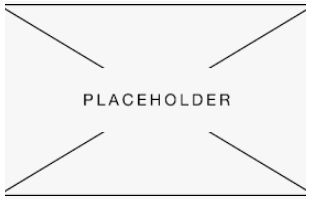
\includegraphics[scale=0.3]{placeholder}\par
    \noindent Commentaire en-dessous du diagramme\par
  \end{center} % or flushleft or flushright

  % Option 1. A single question with no breakdown into parts
  \medskip
  \noindent Un seul bloc de paragraphes qui décrit la question.  La valeure maximale de la note entre parentheses carrées à la marge droite de la derniere ligne.\hspace*{\fill} [?]\par
  
\end{question}
